\documentclass{beamer}
\usepackage{graphicx}
\graphicspath{{Figures/}}
\usepackage{amsmath}
\usecolortheme{orchid}
\usepackage{tikz}
\usetikzlibrary{arrows}
\usepackage[T1]{fontenc}
\usepackage{lmodern}

\newtheorem{thm}{Theorem}[section]
\newtheorem{cor}[thm]{Corollary}
\newtheorem{lem}[thm]{Lemma}
\newtheorem{prop}[thm]{Proposition}
\newtheorem{conj}[thm]{Conjecture}

\theoremstyle{definition}
\newtheorem{defn}[thm]{Definition}
\newtheorem{exm}[thm]{Example}

\theoremstyle{remark}
\newtheorem{remark}[thm]{Remark}

\newcommand{\A}{\mathcal{A}}
\newcommand{\QC}{\mathcal{Q}}
\newcommand{\PC}{\mathcal{P}}
\newcommand{\R}{\mathbb{R}}
\newcommand{\Z}{\mathbb{Z}}
\newcommand{\mR}{\mathcal{R}}
\newcommand{\mJ}{\mathcal{J}}
\newcommand{\nl}{\mathnormal{l}}
\newcommand{\wPC}{\widehat{\PC}}
\newcommand{\wQC}{\widehat{\QC}}
\newcommand{\reg}{\mbox{\emph{reg}}}
\newcommand{\syz}{\mbox{\emph{syz}}}
\newcommand{\wDelta}{\widehat{\Delta}}

\title[M2 Splines Package]{M2 Splines Package}
\author{\large{Daniel Bernstein, Michael DiPasquale, Eliana Duarte, Gwyneth Whieldon}}
\institute{\large{M2 Workshop}\\ \normalsize{Boise State University}}
\date[May 30, 2015]{May 30, 2015}

\begin{document}
\frame{\titlepage}

\section{Background}

\begin{frame}
\frametitle{Piecewise Polynomials}

\begin{itemize}

\item $\PC:$ subdivision of a simply-connected domain $\Omega\subset\R^n$ by convex polytopes (polytopal complex)

\onslide+<2->

\item $C^r(\PC):$ all functions $F:\Omega\rightarrow \R$, continuously differentiable of order $r$, whose restriction to each part of the subdivision $\PC$ is a \textbf{polynomial}.  $F$ is called an $r$-\textbf{spline} (or just a spline).

\onslide+<3->

\item \textbf{Degree} of a spline: max degree of polynomials it restricts to on each piece of the subdivision.

\item $C^r_d(\PC):$ $r$-splines of degree $\le d$ on $\PC$

\end{itemize}

\begin{center}
\begin{tabular}{ccc}
\onslide+<4->{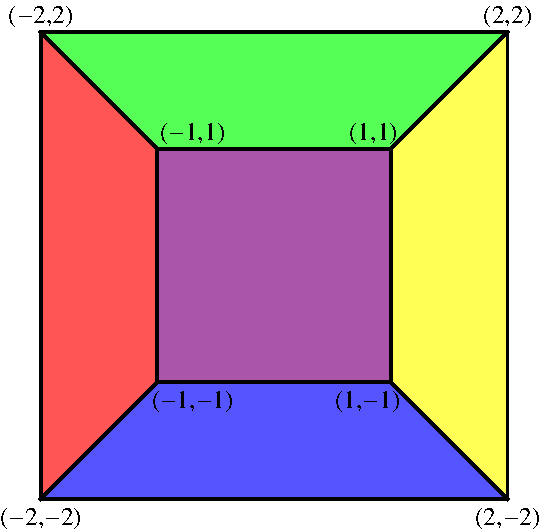
\includegraphics[width=.3\textwidth]{ColorSquareVertexLabelled.pdf}} & \onslide+<5->{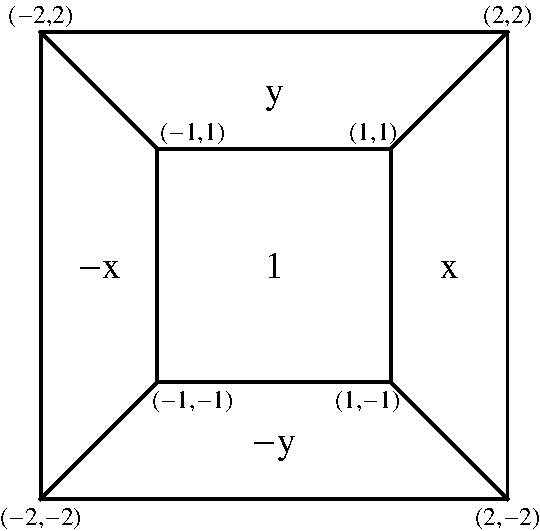
\includegraphics[width=.3\textwidth]{ToySplineVertexLabelled.pdf}} & \onslide+<6->{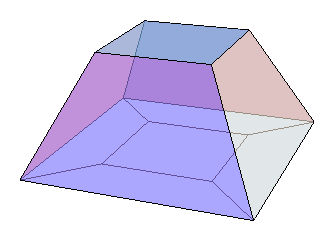
\includegraphics[width=.3\textwidth]{SchlegelCubeNTPL.png}} \\
\onslide+<4->{A Polytopal Complex $\QC$} & \onslide+<5->{A Spline $F\in C^0_1(\QC)$} & \onslide+<6->{Graph of $F$}
\end{tabular}
\end{center}

\end{frame}

\begin{frame}
\frametitle{A More Interesting Example}

\vspace{-150 pt}

\begin{overlayarea}{\textwidth}{40 pt}

\begin{center}
\only<1>{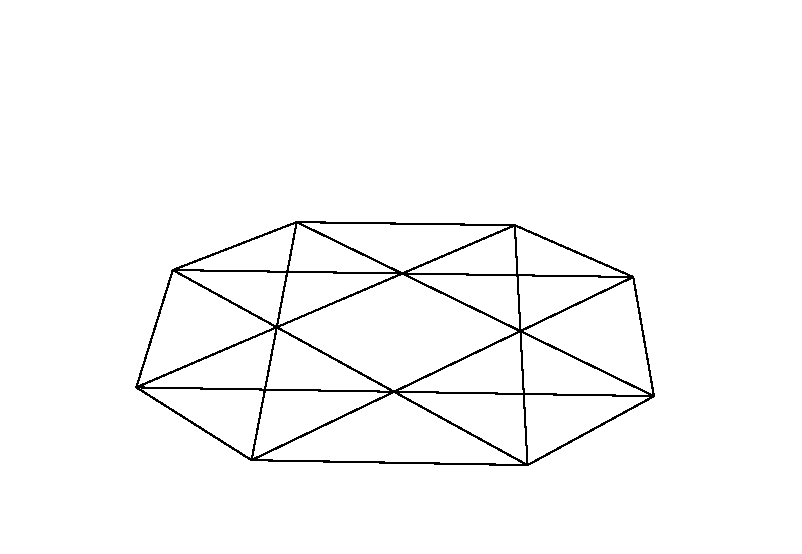
\includegraphics[width=.8\textwidth]{ZPBase.pdf}}
\only<2-4>{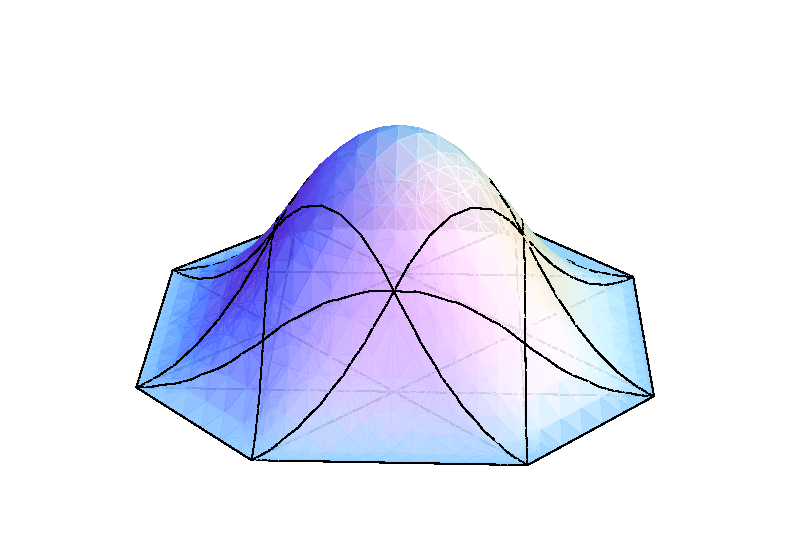
\includegraphics[width=.8\textwidth]{ZP.pdf}}
\end{center}

\vspace{-30 pt}

\begin{itemize}
\item \onslide+<1->{Partition $\PC$ of an octagonal domain $\subset\R^2$}

\item \onslide+<2->{Graph of the \textbf{Zwart-Powell element}: a spline in $C^1_2(\PC)$.}

\item \onslide+<3->{Twenty-seven polynomials fit together to form this spline.}

\item \onslide+<4->{This is an example of a \textbf{box spline}.}
%Used in
%\begin{enumerate}
%\item Construct subdivision surfaces in computer graphics
%\item Signal processing
%\item Computations of polytope volumes, characterizations of hyperplane arrangements
%\item 
%\end{enumerate}
%
%computer graphics, computations of }
\end{itemize}

\end{overlayarea}

\end{frame}

\begin{frame}
\frametitle{Polynomials of ZP Element}

\begin{center}
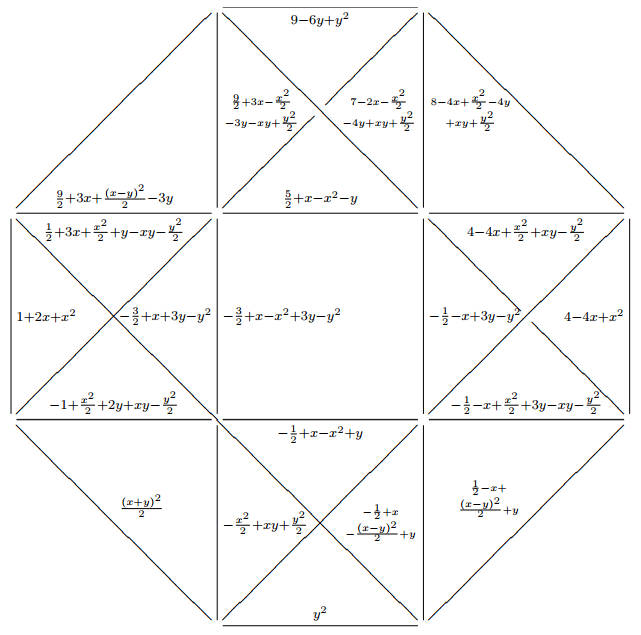
\includegraphics[scale=.45]{ZPPolys.png}

\tiny{Image taken from C. Procesi, `The algebra of the box-spline,' Temple University, 2006.}
\end{center}

\end{frame}

\begin{frame}
\frametitle{Algebraic Criterion}

\begin{columns}

\column{.5\textwidth}

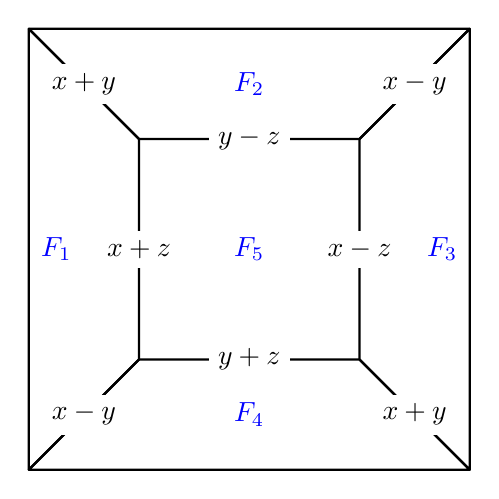
\begin{tikzpicture}[scale=.7]

\tikzstyle{gry}=[thick,join=round]

\node[shape=coordinate] (idr) at (2,-2){};
\node[shape=coordinate] (iur) at (2,2){};
\node[shape=coordinate] (idl) at (-2,-2){};
\node[shape=coordinate] (iul) at (-2,2){};
\node[shape=coordinate] (odr) at (4,-4){};
\node[shape=coordinate] (our) at (4,4){};
\node[shape=coordinate] (odl) at (-4,-4){};
\node[shape=coordinate] (oul) at (-4,4){};

\draw[gry] (idl)--(odl)--(oul)--(iul)--cycle;
\draw[gry] (idr)--(odr)--(odl)--(idl)--cycle;
\draw[gry] (iur)--(our)--(odr)--(idr)--cycle;
\draw[gry] (iul)--(oul)--(our)--(iur)--cycle;

\node[fill=white,fill opacity=1] at (-3,-3) {$x-y$};
\node[fill=white,fill opacity=1] at (-3,3) {$x+y$};
\node[fill=white,fill opacity=1] at (3,3) {$x-y$};
\node[fill=white,fill opacity=1] at (3,-3) {$x+y$};
\node[fill=white,fill opacity=1] at (0,-2) {$y+z$};
\node[fill=white,fill opacity=1] at (-2,0) {$x+z$};
\node[fill=white,fill opacity=1] at (0,2) {$y-z$};
\node[fill=white,fill opacity=1] at (2,0) {$x-z$};

\node[blue] at (-3.5,0) {$F_1$};
\node[blue] at (0,3) {$F_2$};
\node[blue] at (3.5,0) {$F_3$};
\node[blue] at (0,-3) {$F_4$};
\node[blue] at (0,0) {$F_5$};


\end{tikzpicture}

\pause

\column{.5\textwidth}
$(F_1,F_2,F_3,F_4,F_5)\in C^r(\widehat{\QC})\iff$
there are $f_1,\ldots,f_8\in S=\R[x,y,z]$ s.t.
\[
\begin{array}{c}
F_1-F_2=f_1(x+y)^{r+1} \\ F_2-F_3=f_2(x-y)^{r+1} \\
F_3-F_4=f_3(x+y)^{r+1} \\ F_4-F_1=f_4(x-y)^{r+1}\\
F_1-F_5=f_5(x+z)^{r+1} \\ F_2-F_5=f_6(y-z)^{r+1}\\
F_3-F_5=f_7(x-z)^{r+1} \\ F_4-F_5=f_8(y+z)^{r+1}
\end{array}
\]
\end{columns}

\end{frame}

\begin{frame}
\frametitle{Spline Matrix for $C^r(\widehat{\QC})$}

\begin{columns}

\column{.3\textwidth}

\centering

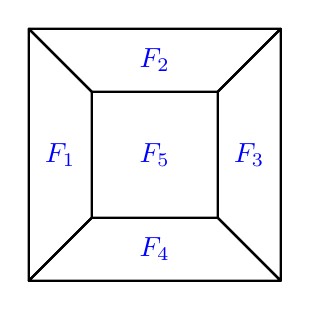
\begin{tikzpicture}[scale=.4]

\tikzstyle{gry}=[thick,join=round]

\node[shape=coordinate] (idr) at (2,-2){};
\node[shape=coordinate] (iur) at (2,2){};
\node[shape=coordinate] (idl) at (-2,-2){};
\node[shape=coordinate] (iul) at (-2,2){};
\node[shape=coordinate] (odr) at (4,-4){};
\node[shape=coordinate] (our) at (4,4){};
\node[shape=coordinate] (odl) at (-4,-4){};
\node[shape=coordinate] (oul) at (-4,4){};

\draw[gry] (idl)--(odl)--(oul)--(iul)--cycle;
\draw[gry] (idr)--(odr)--(odl)--(idl)--cycle;
\draw[gry] (iur)--(our)--(odr)--(idr)--cycle;
\draw[gry] (iul)--(oul)--(our)--(iur)--cycle;

\node[blue] at (-3,0) {$F_1$};
\node[blue] at (0,3) {$F_2$};
\node[blue] at (3,0) {$F_3$};
\node[blue] at (0,-3) {$F_4$};
\node[blue] at (0,0) {$F_5$};

\end{tikzpicture}

\column{.7\textwidth}

\vspace{10 pt}

\centering

$(F_1,F_2,F_3,F_4,F_5)\in C^r(\widehat{\QC})\iff$
there are $f_1,\ldots,f_8$ so that

\end{columns}

\pause

\tiny
\arraycolsep=.3pt % default: 5pt
\medmuskip = .3mu % default: 4mu plus 2mu minus 4mu

\[
\hspace{-.5cm}
\left(
\begin{array}{ccccccccccccc}
 1 & -1 & 0 & 0 & 0 & (x-y)^{r+1} & 0 & 0 & 0 & 0 & 0 & 0 & 0 \\
 0 & 1 & -1 & 0 & 0 & 0 & (x+y)^{r+1} & 0 & 0 & 0 & 0 & 0 & 0 \\
 0 & 0 & 1 & -1 & 0 & 0 & 0 & (x-y)^{r+1} & 0 & 0 & 0 & 0 & 0 \\
 -1 & 0 & 0 & 1 & 0 & 0 & 0 & 0 & (x+y)^{r+1} & 0 & 0 & 0 & 0 \\
 1 & 0 & 0 & 0 & -1 & 0 & 0 & 0 & 0 & (x+z)^{r+1} & 0 & 0 & 0 \\
 0 & 1 & 0 & 0 & -1 & 0 & 0 & 0 & 0 & 0 & (y-z)^{r+1} & 0 & 0 \\
 0 & 0 & 1 & 0 & -1 & 0 & 0 & 0 & 0 & 0 & 0 & (x-z)^{r+1} & 0 \\
 0 & 0 & 0 & 1 & -1 & 0 & 0 & 0 & 0 & 0 & 0 & 0 & (x+z)^{r+1} \\
\end{array}
\right)
\left(
\begin{array}{c}
F_1\\
F_2\\
F_3\\
F_4\\
F_5\\
-f_1\\
-f_2\\
-f_3\\
-f_4\\
-f_5\\
-f_6\\
-f_7\\
-f_8
\end{array}
\right)
=0
\]

\end{frame}

\begin{frame}
\frametitle{The Dimension Question}

Key Fact: $C^r_d(\PC)$ is a finite dimensional real vector space.

\begin{minipage}{.3\textwidth}
\onslide+<2->{
A basis for $C^0_1(\QC)$
is shown at right.}
\vspace{10 pt}
\onslide+<3->{
$\mbox{dim}_\R C^0_1(\QC)=4$}
\end{minipage}
\begin{minipage}{.5\textwidth}
\onslide+<3->{
\begin{tabular}{cc}
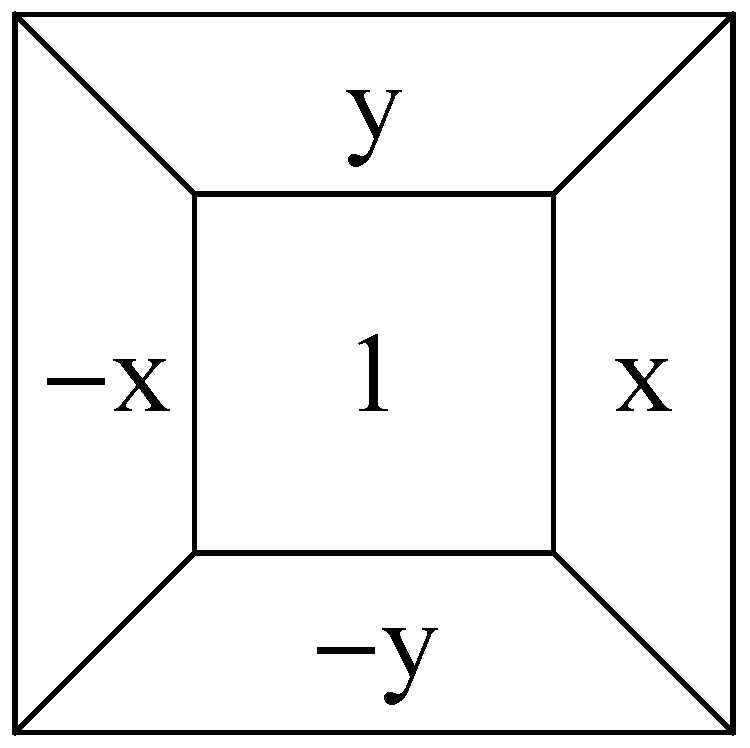
\includegraphics[scale=.23]{ToySpline.pdf} & 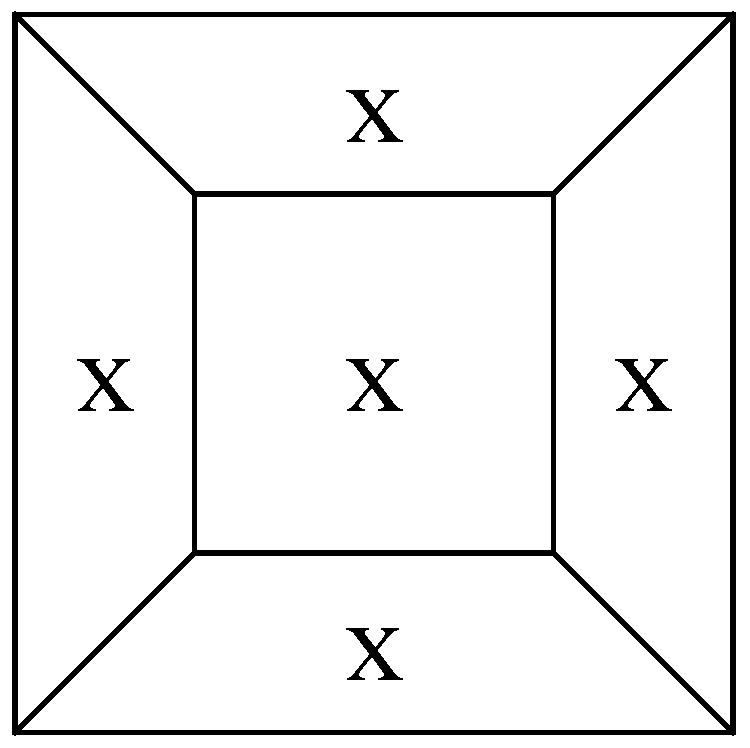
\includegraphics[scale=.23]{ToySplinex.pdf} \\
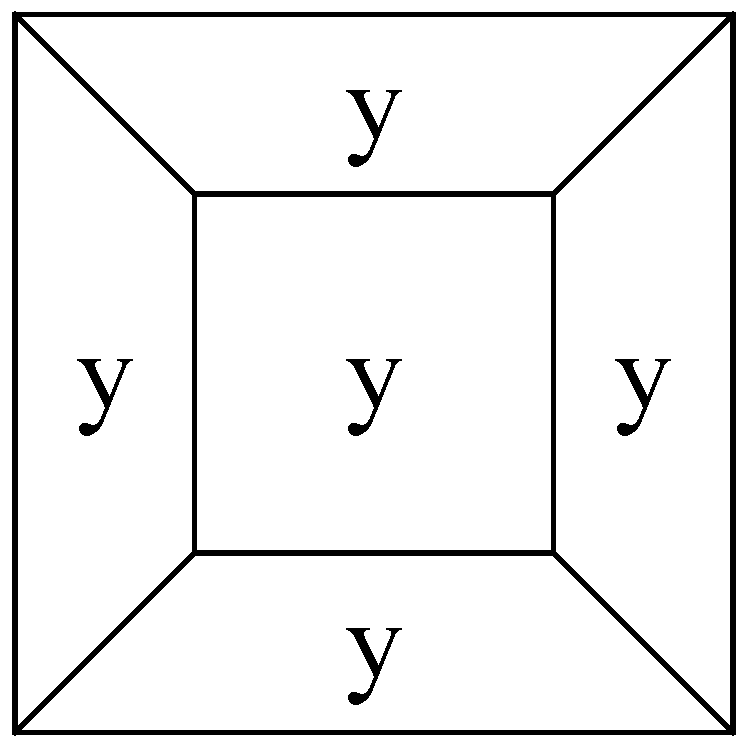
\includegraphics[scale=.23]{ToySpliney.pdf} & 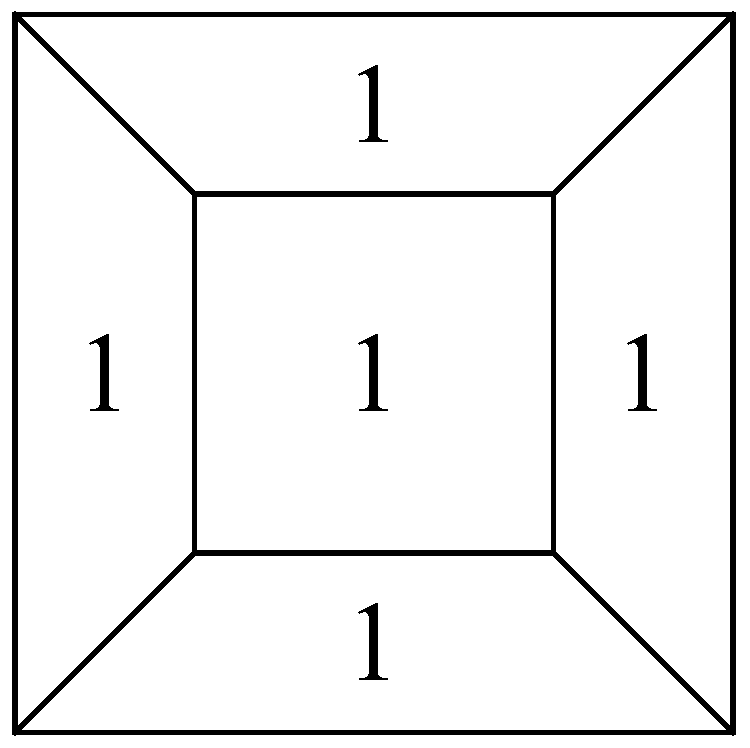
\includegraphics[scale=.23]{ToySpline1.pdf}
\end{tabular}
}
\end{minipage}

\onslide+<4->{
Two central problems in approximation theory:
\begin{enumerate}
\item Determine $\dim C^r_d(\PC)$
\item Construct a basis of $C^r_d(\PC)$ with `good' properties
\end{enumerate}
}
\end{frame}

\end{document}